\documentclass[openany,11pt]{book}	
\usepackage{xcolor}
%\definecolor{Sumire}{RGB}{102,50,124}
%\definecolor{Shion}{RGB}{143,119,181}
\definecolor{ecolor}{RGB}{1,126,218}

\usepackage{tikz-cd}
\usepackage{titlesec}
\usepackage{titleps}
\usepackage{tikz}
\usetikzlibrary{arrows.meta}


\newcommand{\chapnumfont}{%
	\fontsize{100}{100}\usefont{T1}{ptm}{b}{n}%
}

\colorlet{chapbgcolor}{gray!75}
\colorlet{chapnumcolor}{black!60}


\newcommand{\chaptitlenumbered}[1]{%
	\begin{tikzpicture}
		\fill[chapbgcolor!70,rounded corners=0pt] (0,2.3) rectangle (\linewidth,0);
		\node[
		align=right,
		anchor=south east,
		inner sep=8pt,
		font=\LARGE\normalfont\bfseries
		] at (0.987\linewidth,0) {\strut#1};
		\node[
		align=right,
		font=\fontsize{60}{62}\usefont{OT1}{ptm}{b}{it},
		text=chapnumcolor
		] at (0.975\linewidth,2.3) {\thechapter};
	\end{tikzpicture}%
}

\newcommand{\chaptitleunnumbered}[1]{%
	\begin{tikzpicture}
		\fill[chapbgcolor!70,rounded corners=0pt] (0,2.3) rectangle (\linewidth,0);
		\node[
		align=right,
		anchor=south east,
		inner sep=8pt,
		font=\huge\normalfont\bfseries
		] at (0.987\linewidth,0) {\strut#1};
	\end{tikzpicture}%
}

\usepackage{titlesec}

\titleformat{name=\chapter}[display]
{\normalfont\huge\bfseries\sffamily}
{}
{40pt}
{\chaptitlenumbered}
\titleformat{name=\chapter,numberless}[display]
{\normalfont\huge\bfseries\sffamily}
{}
{25pt}
{\chaptitleunnumbered}
\titlespacing*{\chapter}
{0pt}
{-126pt}
{33pt}

\titleformat{\section}
{\normalfont\Large\bfseries\color{red}}
{{\mdseries\S}\ \thesection}{.5em}{}

\titleformat{\subsection}
{\normalfont\large\bfseries\color{red}}
{{\mdseries\S}\ \thesubsection}{.5em}{}

\setlength\headheight{15pt}

\usepackage{dsfont}

\renewcommand{\baselinestretch}{1.25}

\renewcommand\sectionmark[1]{%
	\markright{\thesection\quad #1}}

% \usepackage{indentfirst}
\setlength{\parindent}{0pt}
% 无首航缩进

\usepackage{parskip}
\setlength{\parskip}{0.5\baselineskip} % 设置段落间距为两倍的基线间距,即空两行

\usepackage{xeCJK}
%\setCJKmainfont{PingFangSC-Regular}


%设定字体

%% \setCJKmainfont[ItalicFont=STKaiti]{Source Han Serif CN}
%% 为思源宋体

%\setCJKmainfont[BoldFont=黑体, ItalicFont=STKaiti]{Source Han Serif CN}
%% 为中易黑体

%% \setCJKsansfont{Source Han Sans CN}
%% \setCJKmonofont{Source Han Sans CN}
%% \setCJKfamilyfont{boldsong}{Source Han Serif CN Heavy}
%\normalspacedchars{*}
%数学式
\usepackage{mathtools,extarrows,amsfonts,amssymb,bm,mathrsfs} %数学式宏包, 更多箭头, 黑板体等数学字体,leqslant等符号
\usepackage{amsthm} %定理环境

\allowdisplaybreaks
\usepackage{ulem}
% 下划线

\DeclareMathOperator{\rad}{rad}
\DeclareMathOperator{\diam}{diam}
\DeclareMathOperator{\fin}{fin}
\DeclareMathOperator{\esssup}{ess,sup}
\DeclareMathOperator{\conv}{Conv}
\DeclareMathOperator{\Span}{span} %% 因为\span已经在宏中定义, 这里使用大写的\Span来表示线性张成
\DeclareMathOperator{\cont}{Cont} %% 表示函数的连续点
\DeclareMathOperator{\diag}{diag}
\DeclareMathOperator{\codim}{codim}
\DeclareMathOperator{\convba}{Convba}


\newcommand{\me}{\ensuremath{\mathrm{e}}}
\newcommand{\imag}{\mathrm{i}}
\newcommand{\Star}[1]{#1^{*}}
\newcommand{\1}{\mathds{1}}
\newcommand{\supp}{\mathrm{supp},}

%% \C已被定义, 重定义在交叉引用部分
\newcommand{\R}{\ensuremath{\mathbb{R}}}
\newcommand{\J}{\ensuremath{\mathbb{J}}}
\newcommand{\Q}{\ensuremath{\mathbb{Q}}}
\newcommand{\Z}{\ensuremath{\mathbb{Z}}}
\newcommand{\N}{\ensuremath{\mathbb{N}}}
\newcommand{\K}{\ensuremath{\mathbb{K}}}
\newcommand{\Zo}{\ensuremath{\mathbb{Z}_{\geqslant 0}}} % 非负整数集
\newcommand{\Zi}{\ensuremath{\mathbb{Z}_{\geqslant 1}}} % 正整数集
\newcommand{\id}{\mathrm{id}}
\newcommand{\im}{\mathrm{im},}                         % 映射的像

\newcommand{\CA}{\mathcal{A}}
\newcommand{\CB}{\mathcal{B}}
\newcommand{\CF}{\mathcal{F}}
\newcommand{\CG}{\mathcal{G}}
\newcommand{\CH}{\mathcal{H}}
\newcommand{\CK}{\mathcal{K}}
\newcommand{\CL}{\mathcal{L}}
\newcommand{\CN}{\mathcal{N}}

\newcommand{\FB}{\mathfrak{B}}

\renewcommand{\Re}{\mathrm{Re,}}
\renewcommand{\Im}{\mathrm{Im,}}
\newcommand{\sgn}{\mathrm{sgn},}
\newcommand{\diff}{,\mathrm{d}}

\newcommand{\Fs}{\ensuremath{\CF_{\sigma}}}
\newcommand{\Gd}{\ensuremath{\CG_{\delta}}}
\newcommand{\Fr}{\ensuremath{\CF_{r}}}


%\usepackage{tasks}
%\NewTasks[counter-format=(tsk[1]), item-indent=2em, label-offset=1em, label-align=right]{lpbn}
%\NewTasks[counter-format=(tsk[a]), item-indent=2em, label-offset=1em]{alpbn}
%\NewTasks[counter-format=tsk[A].]{xrze}[*]

%版式
\usepackage[a4paper,left=2.5cm,right=2.5cm,top=2.5cm,bottom=2cm]{geometry} %边距
%\usepackage[a4paper,left=1.8cm,right=3.2cm,top=2.5cm,bottom=2cm]{geometry} %当打印时使用此选项
\setlength{\headheight}{13pt}
\usepackage{pifont}		% 带圈数字
\usepackage{fancyhdr} 	% 页眉页脚
\pagestyle{fancy}
\fancyhf{}
\fancyhead[OL]{\Roman \nouppercase\rightmark}
\fancyhead[ER]{\Roman \nouppercase\leftmark}
\fancyhead[OR,EL]{\thepage}
\fancyfoot[C]{}
\usepackage{tocbibind}
\usepackage{imakeidx}

%辅助
\usepackage{array,diagbox,booktabs,tabularx} 
%数组环境, 表格中可以添加对角线, 可以调整表格中线的宽度, 可以控制表格宽度并使其自动换行
\usepackage{enumitem} % 继承并扩展了enumerate宏包的功能
% 对itemize环境进行设置
\setlist[itemize]{
	labelindent=\parindent, % 项目符号缩进一个缩进距离
	labelsep=0.5em, % 内容和项目符号之间的间距设为1em,可按需调整
	leftmargin=2em, 
	noitemsep, % 去除列表项之间的额外垂直间距
	itemindent=0pt % 列表项内容不额外缩进
}
\setlength{\topsep}{0ex} % 列表到上下文的垂直距离

%交叉引用
\usepackage{nameref}
\usepackage{prettyref}
\usepackage[colorlinks, linkcolor=red,citecolor=red,urlcolor=black]{hyperref}

\usepackage{graphicx}
\newcommand{\C}{\ensuremath{\mathbb{C}}} 
%浮动体
\usepackage{caption} %使用浮动体标题
\usepackage{subfig} %子浮动体

% 新定义计数器
\newcounter{FA}[chapter]
\renewcommand{\theFA}{\thechapter.\arabic{FA}}

%新定义定理环境
\theoremstyle{plain}
%\theoremstyle{Thm}
\newtheorem{theorem}[FA]{Theorem}
\newtheorem*{theoremn}{Theorem}
\newtheorem{lemma}[FA]{Lemma}
\newtheorem{remark}[FA]{Remark}
\newtheorem*{remarkn}{Remark}
\newtheorem*{solution}{Solution}
\newtheorem{exercise}{Exercise}
\newtheorem{problem}{Problem}
\newtheorem{definition}[FA]{Definition}
\newtheorem*{definitionn}{Definition}
\newtheorem{corollary}[FA]{Corollary}
\newtheorem{example}[FA]{Example}
\newtheorem{proposition}[FA]{Proposition}
\newtheorem{extraexample}{Extraexample}
\newtheorem*{lemman}{Lemma} %
\newtheorem*{propositionn}{Proposition}
\newtheorem*{corollaryn}{Corollary} 

\newtheoremstyle{plain}{\topsep}{\topsep}{\normalfont}{}{%
	\color{blue}\bfseries}{}{%
	0.5em}{%
	\thmname{#1}\thmnumber{ #2}\thmnote{ (#3)}}

\renewcommand*{\proofname}{%
	\normalfont\bfseries\color{blue} Proof}

%新定义命令
\newcommand{\abs}[1]{\ensuremath{\left| #1 \right| }}
\newcommand{\norm}[1]{\ensuremath{\left\| #1 \right\|}}
\newcommand{\tabs}[1]{\ensuremath{\lvert #1\rvert}}
\newcommand{\tnorm}[1]{\ensuremath{\lVert #1\rVert}}
\newcommand{\Babs}[1]{\ensuremath{\Big| #1 \Big| }}
\newcommand{\Bnorm}[1]{\ensuremath{\Big\| #1 \Big\|}}
\newcommand{\lrangle}[1]{\left\langle #1 \right\rangle}
\newcommand{\degree}{\ensuremath{^{\circ}}}
\newcommand{\sm}{\ensuremath{\setminus}}
\newcommand{\baro}[1]{\overline{#1}}
\newcommand{\weakto}{\ensuremath{\overset{w.}{\longrightarrow}}}
\newcommand{\sweakto}{\ensuremath{\overset{\Star{w.}}{\longrightarrow}}}
\newcommand{\seq}[2][n]{\ensuremath{#2_{1}, #2_{2}, \dots, #2_{#1}}}
\renewcommand{\thefootnote}{$\sharp$\arabic{footnote}}
%\renewcommand{\labelenumi}{(\theenumi)}


\usepackage{float}
\usepackage{pdfpages}

\makeindex[intoc]
\renewcommand{\qedsymbol}{$\blacksquare$}
\pagestyle{plain}

\usepackage{pgfplots}
% 图画
\addtolength{\jot}{0.5em}

% 如果图片没有指定后缀, 依次按下列顺序搜索
\DeclareGraphicsExtensions{.pdf,.eps,.jpg,.png}
% 设置图表搜索路径, 可以给图表文件夹取如下名字
\graphicspath{{figures/}{figure/}{pictures/}%
	{picture/}{pic/}{pics/}{image/}{images/}}

\renewcommand{\contentsname}{Content}
\usepackage{algorithm}
\usepackage{algpseudocode}

% INPUT和OUTPUT
\renewcommand{\algorithmicrequire}{\textbf{Input:}}
\renewcommand{\algorithmicensure}{\textbf{Output:}}

\renewcommand{\bibname}{References}
% 修改参考文献标题



\usepackage{tcolorbox}

\tcbuselibrary{breakable}
\newtcolorbox{pbox}[1][]{
	colframe=gray!85, % 边框颜色
	colback=white,       % 背景色
	title={\textbf{#1}}, % 标题文本
	% before upper={\setlength{\parindent}{1.5em}}, % 设置首行缩进
	% before lower={\setlength{\parindent}{1.5em}}, % 下面首行不缩进
	breakable,           % 允许跨页
}


\usepackage{svg}

\begin{document}

\chapter{回归问题}

参考:https://zh-v2.d2l.ai/

回归(regression)是能为一个或多个自变量与因变量之间关系建模的一类方法。

在自然科学和社会科学领域,回归经常用来表示输入和输出之间的关系。

在机器学习领域中的大多数任务通常都与预测(prediction)有关。

当我们想预测一个数值时,就会涉及到回归问题。

常见的例子包括:预测价格(房屋、股票等)、预测住院时间(针对住院病人等)、预测需求(零售销量等)。

但不是所有的预测都是回归问题。


\section{线性回归的基本元素}

线性回归(linear regression)可以追溯到19世纪初,它在回归的各种标准工具中最简单而且最流行。

线性回归基于几个简单的假设:

\begin{itemize}
	\item 自变量$\mathbf{x}$和因变量$y$之间的关系是线性的。即$y$可以表示为$\mathbf{x}$中元素的加权和,这里通常允许包含观测值的一些噪声;
	\item 任何噪声都比较正常,如噪声遵循正态分布。
\end{itemize}

~\\
{\color{red}根据房屋的面积(平方英尺)和房龄(年)来估算房屋价格(美元)}

为了开发一个能预测房价的模型,我们需要收集一个真实的数据集。

这个数据集包括了房屋的销售价格、面积和房龄。

~\\
在机器学习的术语中:
\begin{itemize}
	\item 数据集称为训练数据集(training data set)或 训练集(training set)。
	\item 每行数据(比如一次房屋交易相对应的数据)称为样本(sample),也可以称为数据点(data point)或数据样本(data instance)。
	\item 预测的目标(比如预测房屋价格)称为标签(label)或目标(target)。
	\item 预测所依据的自变量(面积和房龄)称为特征(feature)或协变量(covariate)。
	\item 我们使用$n$来表示数据集中的样本数。对索引为$i$的样本,其输入表示为$\mathbf{x}^{(i)} = [x_1^{(i)}, x_2^{(i)}]^\top$,其对应的标签是$y^{(i)}$。
\end{itemize}

\section{线性模型}


线性假设是指目标(房屋价格)可以表示为特征(面积和房龄)的加权和,如下面的式子:
$$\mathrm{price} = w_{\mathrm{area}} \cdot \mathrm{area} + w_{\mathrm{age}} \cdot \mathrm{age} + b.$$
其中的$w_{\mathrm{area}}$和$w_{\mathrm{age}}$称为权重(weight),权重决定了每个特征对我们预测值的影响。

$b$称为偏置(bias)、偏移量(offset)或截距(intercept)。

偏置是指当所有特征都取值为0时,预测值应该为多少。


~\\
{\color{red} 即使现实中不会有任何房子的面积是0或房龄正好是0年,我们仍然需要偏置项。}

如果没有偏置项,我们模型的表达能力将受到限制。

严格来说,是输入特征的一个 仿射变换(affine transformation)。

仿射变换的特点是通过加权和对特征进行线性变换(linear transformation),并通过偏置项来进行平移(translation)。

~\\
给定一个数据集,我们的目标是寻找模型的权重$\mathbf{w}$和偏置$b$,
使得根据模型做出的预测大体符合数据里的真实价格。

输出的预测值由输入特征通过线性模型的仿射变换决定,仿射变换由所选权重和偏置确定。

~\\
在机器学习领域,我们通常使用的是{\color{red} 高维数据集},建模时采用线性代数表示法会比较方便。
当我们的输入包含$d$个特征时,我们将预测结果$\hat{y}$
(通常使用“尖角”符号表示$y$的估计值)表示为:
$$\hat{y} = w_1  x_1 + ... + w_d  x_d + b.$$
将所有特征放到向量$\mathbf{x} \in \mathbb{R}^d$中,
并将所有权重放到向量$\mathbf{w} \in \mathbb{R}^d$中,
我们可以用点积形式来简洁地表达模型:
$$\hat{y} = \mathbf{w}^\top \mathbf{x} + b.$$
向量$\mathbf{x}$对应于单个数据样本的特征。
用符号表示的矩阵$\mathbf{X} \in \mathbb{R}^{n \times d}$
可以很方便地引用我们整个数据集的$n$个样本。
其中,$\mathbf{X}$的每一行是一个样本,每一列是一种特征。

对于特征集合$\mathbf{X}$,预测值$\hat{\mathbf{y}} \in \mathbb{R}^n$
可以通过矩阵-向量乘法表示为:
$${\hat{\mathbf{y}}} = \mathbf{X} \mathbf{w} + b$$

~\\
给定训练数据特征$\mathbf{X}$和对应的已知标签$\mathbf{y}$,
线性回归的目标是找到一组权重向量$\mathbf{w}$和偏置$b$:

当给定从$\mathbf{X}$的同分布中取样的新样本特征时,
这组权重向量和偏置能够使得新样本预测标签的误差尽可能小。

虽然我们相信给定$\mathbf{x}$预测$y$的最佳模型会是线性的,
但我们很难找到一个有$n$个样本的真实数据集,其中对于所有的$1 \leq i \leq n$,$y^{(i)}$完全等于$\mathbf{w}^\top \mathbf{x}^{(i)}+b$。

无论我们使用什么手段来观察特征$\mathbf{X}$和标签$\mathbf{y}$,
都可能会出现少量的观测误差。

因此,即使确信特征与标签的潜在关系是线性的,
我们也会加入一个噪声项来考虑观测误差带来的影响。

在开始寻找最好的模型参数(model parameters)$\mathbf{w}$和$b$之前,我们还需要两个东西:
\begin{itemize}
	\item 一种模型质量的度量方式;
	
	\item 一种能够更新模型以提高模型预测质量的方法。
\end{itemize}

\section{损失函数}

在我们开始考虑如何用模型拟合(fit)数据之前,我们需要确定一个拟合程度的度量。

损失函数(loss function)能够量化目标的实际值与预测值之间的差距。

通常我们会选择非负数作为损失,且数值越小表示损失越小,完美预测时的损失为0。

回归问题中最常用的损失函数是平方误差函数。

当样本$i$的预测值为$\hat{y}^{(i)}$,其相应的真实标签为$y^{(i)}$时,
平方误差可以定义为以下公式:
$$l^{(i)}(\mathbf{w}, b) = \frac{1}{2} \left(\hat{y}^{(i)} - y^{(i)}\right)^2.$$
常数$\frac{1}{2}$不会带来本质的差别,但这样在形式上稍微简单一些
(因为当我们对损失函数求导后常数系数为1)。

由于训练数据集并不受我们控制,所以经验误差只是关于模型参数的函数。

~\\
{\color{red} 我们为一维情况下的回归问题绘制图像,}

\begin{figure}
	\centering
	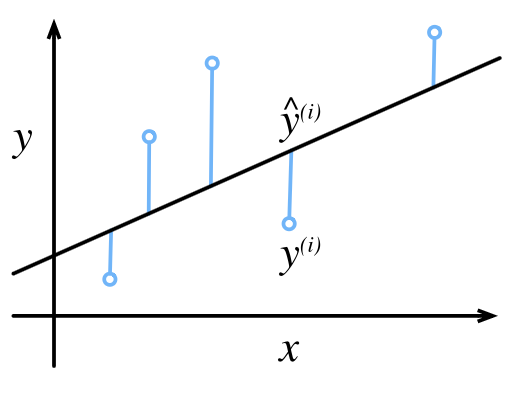
\includegraphics[width=0.5\linewidth]{image.png}
	\label{fig:placeholder}
\end{figure}

由于平方误差函数中的二次方项,
估计值$\hat{y}^{(i)}$和观测值$y^{(i)}$之间较大的差异将导致更大的损失。

为了度量模型在整个数据集上的质量,我们需计算在训练集$n$个样本上的损失均值(也等价于求和)。
$$L(\mathbf{w}, b) =\frac{1}{n}\sum_{i=1}^n l^{(i)}(\mathbf{w}, b) =\frac{1}{n} \sum_{i=1}^n \frac{1}{2}\left(\mathbf{w}^\top \mathbf{x}^{(i)} + b - y^{(i)}\right)^2.$$
在训练模型时,我们希望寻找一组参数($\mathbf{w}, b$),
这组参数能最小化在所有训练样本上的总损失。如下式:
$$(\mathbf{w}, b)= \arg\min_{\mathbf{w}, b}\  L(\mathbf{w}, b).$$



\section{解析解}

线性回归刚好是一个很简单的优化问题。

与我们将在本书中所讲到的其他大部分模型不同,线性回归的解可以用一个公式简单地表达出来,
这类解叫作解析解(analytical solution)。

首先,我们将偏置$b$合并到参数$\mathbf{w}$中,合并方法是在包含所有参数的矩阵中附加一列。

我们的预测问题是最小化$\|\mathbf{y} - \mathbf{X}\mathbf{w}\|^2$。
这在损失平面上只有一个临界点,这个临界点对应于整个区域的损失极小点。

将损失关于$\mathbf{w}$的导数设为0,得到解析解:
$$\mathbf{w}= (\mathbf X^\top \mathbf X)^{-1}\mathbf X^\top \mathbf{y}.$$
像线性回归这样的简单问题存在解析解,但并不是所有的问题都存在解析解。

解析解可以进行很好的数学分析,但解析解对问题的限制很严格,导致它无法广泛应用在深度学习里。



\section{随机梯度下降}

即使在我们无法得到解析解的情况下,我们仍然可以有效地训练模型。

在许多任务上,那些难以优化的模型效果要更好。

因此,弄清楚如何训练这些难以优化的模型是非常重要的。

本书中我们用到一种名为梯度下降(gradient descent)的方法,
这种方法几乎可以优化所有深度学习模型。

它通过不断地在损失函数递减的方向上更新参数来降低误差。

梯度下降最简单的用法是计算损失函数(数据集中所有样本的损失均值)
关于模型参数的导数(在这里也可以称为梯度)。

但实际中的执行可能会非常慢:因为在每一次更新参数之前,我们必须遍历整个数据集。

因此,我们通常会在每次需要计算更新的时候随机抽取一小批样本,
这种变体叫做小批量随机梯度下降(minibatch stochastic gradient descent)。

在每次迭代中,我们首先随机抽样一个小批量$\mathcal{B}$,
它是由固定数量的训练样本组成的。

然后,我们计算小批量的平均损失关于模型参数的导数(也可以称为梯度)。

最后,我们将梯度乘以一个预先确定的正数$\eta$,并从当前参数的值中减掉。

算法的步骤如下:
\begin{itemize}
	\item (1)初始化模型参数的值,如随机初始化;
	\item (2)从数据集中随机抽取小批量样本且在负梯度的方向上更新参数,并不断迭代这一步骤。
\end{itemize}
对于平方损失和仿射变换,我们可以明确地写成如下形式:

$$\begin{aligned} \mathbf{w} &\leftarrow \mathbf{w} -   \frac{\eta}{|\mathcal{B}|} \sum_{i \in \mathcal{B}} \partial_{\mathbf{w}} l^{(i)}(\mathbf{w}, b) = \mathbf{w} - \frac{\eta}{|\mathcal{B}|} \sum_{i \in \mathcal{B}} \mathbf{x}^{(i)} \left(\mathbf{w}^\top \mathbf{x}^{(i)} + b - y^{(i)}\right),\\ b &\leftarrow b -  \frac{\eta}{|\mathcal{B}|} \sum_{i \in \mathcal{B}} \partial_b l^{(i)}(\mathbf{w}, b)  = b - \frac{\eta}{|\mathcal{B}|} \sum_{i \in \mathcal{B}} \left(\mathbf{w}^\top \mathbf{x}^{(i)} + b - y^{(i)}\right). \end{aligned}$$
$\mathbf{w}$和$\mathbf{x}$都是向量。

在这里,更优雅的向量表示法比系数表示法(如$w_1, w_2, \ldots, w_d$)更具可读性。

$|\mathcal{B}|$表示每个小批量中的样本数,这也称为批量大小(batch size)。

$\eta$表示学习率(learning rate)。


~\\
批量大小和学习率的值通常是手动预先指定,而不是通过模型训练得到的。

这些可以调整但不在训练过程中更新的参数称为超参数(hyperparameter)。

调参(hyperparameter tuning)是选择超参数的过程。

超参数通常是我们根据训练迭代结果来调整的,
而训练迭代结果是在独立的验证数据集(validation dataset)上评估得到的。

在训练了预先确定的若干迭代次数后(或者直到满足某些其他停止条件后),
我们记录下模型参数的估计值,表示为$\hat{\mathbf{w}}, \hat{b}$。

但是,即使我们的函数确实是线性的且无噪声,这些估计值也不会使损失函数真正地达到最小值。

因为算法会使得损失向最小值缓慢收敛,但却不能在有限的步数内非常精确地达到最小值。





\chapter{分类问题}
参考:https://zh-v2.d2l.ai/

分类问题:不是问“多少”,而是问“哪一个”:
\begin{itemize}
	\item  某个电子邮件是否属于垃圾邮件文件夹?
	\item  某个用户可能注册或不注册订阅服务?
	\item  某个图像描绘的是驴、狗、猫、还是鸡?
	\item  某人接下来最有可能看哪部电影?
\end{itemize}
通常,机器学习实践者用分类这个词来描述两个有微妙差别的问题:
\begin{itemize}
	\item 我们只对样本的“硬性”类别感兴趣,即属于哪个类别;
	\item 我们希望得到“软性”类别,即得到属于每个类别的概率。
\end{itemize}
这两者的界限往往很模糊。其中的一个原因是:即使我们只关心硬类别,我们仍然使用软类别的模型。(用概率描述离散类别)

~\\
我们从一个图像分类问题开始。{\color{red} 假设每次输入是一个$2\times2$的灰度图像。}

我们可以用一个标量表示每个像素值,每个图像对应四个特征$x_1, x_2, x_3, x_4$。

此外,假设每个图像属于类别“猫”“鸡”和“狗”中的一个。

接下来,我们要选择如何表示标签。
我们有两个明显的选择:最直接的想法是选择$y \in \{1, 2, 3\}$,
其中整数分别代表$\{\text{狗}, \text{猫}, \text{鸡}\}$。
这是在计算机上存储此类信息的有效方法。

~\\
{\color{red} 一种表示分类数据的简单方法:独热编码(one-hot encoding)。}

独热编码是一个向量,它的分量和类别一样多。

类别对应的分量设置为1,其他所有分量设置为0。

在我们的例子中,标签$y$将是一个三维向量,
其中$(1, 0, 0)$对应于“猫”、$(0, 1, 0)$对应于“鸡”、$(0, 0, 1)$对应于“狗”:
$$y \in \{(1, 0, 0), (0, 1, 0), (0, 0, 1)\}.$$


~\\
{\color{red} 现在我们将优化参数以最大化观测数据的概率}

为了得到预测结果,我们将设置一个阈值,如选择具有最大概率的标签。

我们希望模型的输出$\hat{y}_j$可以视为属于类$j$的概率,然后选择具有最大输出值的类别$\operatorname{argmax}_j y_j$作为我们的预测。

例如,如果$\hat{y}_1$、$\hat{y}_2$和$\hat{y}_3$分别为0.1、0.1和0.8,那么我们预测的类别是3,在我们的例子中代表“狗”。


~\\
下面我们为每个输入计算三个未规范化的预测(logit):$o_1$、$o_2$和$o_3$。
$$
\begin{aligned}
	o_1 &= x_1 w_{11} + x_2 w_{12} + x_3 w_{13} + x_4 w_{14} + b_1,\\
	o_2 &= x_1 w_{21} + x_2 w_{22} + x_3 w_{23} + x_4 w_{24} + b_2,\\
	o_3 &= x_1 w_{31} + x_2 w_{32} + x_3 w_{33} + x_4 w_{34} + b_3.
\end{aligned}
$$

然而我们能否将未规范化的预测$o$直接视作我们感兴趣的输出呢?

答案是否定的。

因为将线性层的输出直接视为概率时存在一些问题:

一方面,我们没有限制这些输出数字的总和为1。
另一方面,根据输入的不同,它们可以为负值。

这些违反了中所说的概率基本公理。

要将输出视为概率,我们必须保证在任何数据上的输出都是非负的且总和为1。
此外,我们需要一个训练的目标函数,来激励模型精准地估计概率。

例如,
在分类器输出0.5的所有样本中,我们希望这些样本是刚好有一半实际上属于预测的类别。

这个属性叫做校准(calibration)。


\section{softmax}

softmax函数能够将未规范化的预测变换为非负数并且总和为1,同时让模型保持
可导的性质。

为了完成这一目标,我们首先对每个未规范化的预测求幂,这样可以确保输出非负。

为了确保最终输出的概率值总和为1,我们再让每个求幂后的结果除以它们的总和。如下式:
$$\hat{\mathbf{y}} = \mathrm{softmax}(\mathbf{o})\quad \text{其中}\quad \hat{y}_j = \frac{\exp(o_j)}{\sum_k \exp(o_k)}$$
这里,对于所有的$j$总有$0 \leq \hat{y}_j \leq 1$。

因此,$\hat{\mathbf{y}}$可以视为一个正确的概率分布。

softmax运算不会改变未规范化的预测$\mathbf{o}$之间的大小次序,只会确定分配给每个类别的概率。

因此,在预测过程中,我们仍然可以用下式来选择最有可能的类别。
$$
\operatorname{argmax}_j \hat y_j = \operatorname{argmax}_j o_j.
$$
尽管softmax是一个非线性函数,但softmax回归的输出仍然由输入特征的仿射变换决定。

因此,softmax回归是一个线性模型(linear model)。


\section{损失函数}

对于任何标签$\mathbf{y}$和模型预测$\hat{\mathbf{y}}$,损失函数为:

$$ l(\mathbf{y}, \hat{\mathbf{y}}) = - \sum_{j=1}^q y_j \log \hat{y}_j. $$

损失函数被称为交叉熵损失(cross-entropy loss)。

由于$\mathbf{y}$是一个长度为$q$的独热编码向量,所以除了一个项以外的所有项$j$都消失了。

由于所有$\hat{y}_j$都是预测的概率,所以它们的对数永远不会大于$0$。

因此,如果正确地预测实际标签,即如果实际标签$P(\mathbf{y} \mid \mathbf{x})=1$,则损失函数不能进一步最小化。

注意,这往往是不可能的。

例如,数据集中可能存在标签噪声(比如某些样本可能被误标),或输入特征没有足够的信息来完美地对每一个样本分类。


\section{softmax及其导数}
由于softmax和相关的损失函数很常见,因此我们需要更好地理解它的计算方式。

利用softmax的定义,我们得到:
$$
\begin{aligned}
	l(\mathbf{y}, \hat{\mathbf{y}}) &=  - \sum_{j=1}^q y_j \log \frac{\exp(o_j)}{\sum_{k=1}^q \exp(o_k)} \\
	&= \sum_{j=1}^q y_j \log \sum_{k=1}^q \exp(o_k) - \sum_{j=1}^q y_j o_j\\
	&= \log \sum_{k=1}^q \exp(o_k) - \sum_{j=1}^q y_j o_j.
\end{aligned}
$$
考虑相对于任何未规范化的预测$o_j$的导数,我们得到:
$$
\partial_{o_j} l(\mathbf{y}, \hat{\mathbf{y}}) = \frac{\exp(o_j)}{\sum_{k=1}^q \exp(o_k)} - y_j = \mathrm{softmax}(\mathbf{o})_j - y_j.
$$
换句话说,导数是我们softmax模型分配的概率与实际发生的情况(由独热标签向量表示)之间的差异。

从这个意义上讲,这与我们在回归中看到的非常相似,其中梯度是观测值$y$和估计值$\hat{y}$之间的差异。

\end{document}



% \bibliographystyle{plain} 
% \bibliography{content/ref.bib}
% 参考文献
\end{document}

